\documentclass[12pt,letterpaper]{article}
\usepackage[margin=0.6in,top=0.7in,bottom=0.62in,headheight=15pt,headsep=15pt,footskip=20pt]{geometry}
\usepackage[T1]{fontenc}
\usepackage{lmodern,tikz,fancyhdr,xcolor}
\usetikzlibrary{arrows.meta}
\renewcommand\familydefault{\sfdefault}
\pagestyle{fancy}
\fancyhf{}
\fancyhead[L]{\small Week 84 / Public knowledge / Grades 2--5}
\fancyfoot[L]{\footnotesize Bellingham Math Circle / Week 84 / W84-PK-draft-v2}
\fancyfoot[R]{\footnotesize\thepage}
\renewcommand\headrulewidth{0.4pt}
\renewcommand\footrulewidth{0pt}
\setlength\parindent{0pt}
\setlength\parskip{9pt}
\pdfinfoomitdate=1
\pdfsuppressptexinfo=15
\pdftrailerid{}
\definecolor{hatblue}{RGB}{40,98,171}
\definecolor{hatred}{RGB}{193,70,67}
\definecolor{lightgray}{RGB}{240,240,240}
\newcommand\problem[2]{\textbf{Problem #1:} #2\par}
\newcommand\yn[3]{\node[draw,rounded corners=2pt,minimum width=#3 cm,minimum height=0.62cm,font=\bfseries] at (#1) {#2};}
\newcommand\hatdisk[3]{\ifnum#3=1\fill[hatblue] (#1,#2) circle (0.27);\node[text=white,font=\bfseries] at (#1,#2) {B};\else\fill[hatred] (#1,#2) circle (0.27);\node[text=white,font=\bfseries] at (#1,#2) {R};\fi}
\newcommand\tinydeal[3]{\node[font=\small] at (#1,#2) {#3};}
\newcommand\transcript[6]{%
 \draw[rounded corners=3pt] (#1,#2) rectangle ++(8.05,-2.9);
 \node[anchor=west,font=\bfseries\small] at (#1+0.3,#2-0.38) {Conversation #3};
 \foreach \i/\reply in {1/#4,2/#5,3/#6}{\node[anchor=west,font=\small] at (#1+0.4,#2-0.38-0.7*\i) {\i\quad \reply};}}
\begin{document}
\fontsize{13}{16}\selectfont
\raggedright
Each person sees only their own YES or NO card. Everyone knows the cards can be dealt in any way.

In order, people 1, 2, 3 answer ``Does everyone want a cup?'' Say YES or NO when the cards and earlier answers settle it. Otherwise say NOT YET.

With two people, hearing the first answer changes the possibilities:

\begin{center}
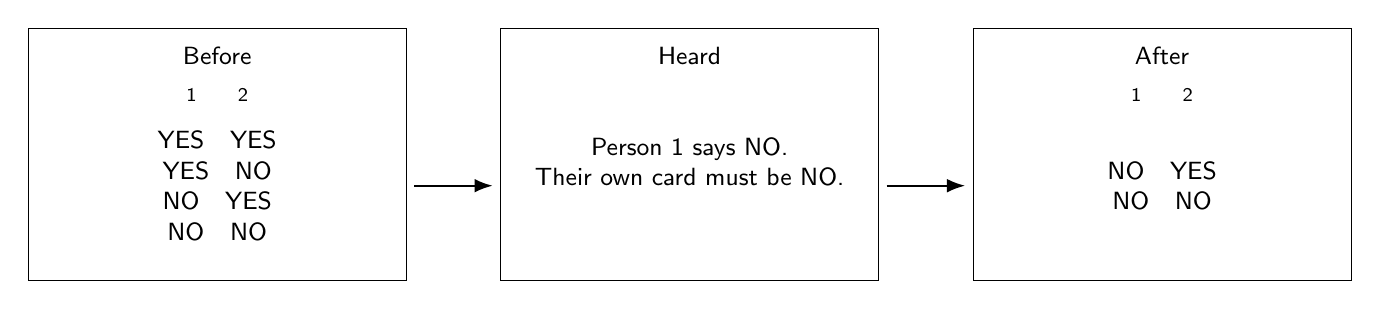
\begin{tikzpicture}[x=1cm,y=1cm,>=Latex]
 \draw (0,0) rectangle (4.8,3.2);\draw (6,0) rectangle (10.8,3.2);\draw (12,0) rectangle (16.8,3.2);
 \node[font=\small] at (2.4,2.85) {Before};\node[font=\small] at (8.4,2.85) {Heard};\node[font=\small] at (14.4,2.85) {After};
 \node[font=\scriptsize] at (2.4,2.35) {1\qquad 2};\node[font=\scriptsize] at (14.4,2.35) {1\qquad 2};
 \node[align=center,font=\small] at (2.4,1.2) {YES\quad YES\\YES\quad NO\\NO\quad YES\\NO\quad NO};
 \node[align=center,font=\small] at (8.4,1.5) {Person 1 says NO.\\Their own card must be NO.};
 \node[align=center,font=\small] at (14.4,1.2) {NO\quad YES\\NO\quad NO};
 \draw[->,thick] (4.9,1.2)--(5.9,1.2);\draw[->,thick] (10.9,1.2)--(11.9,1.2);
\end{tikzpicture}
\end{center}

\problem{1}{Make every YES/NO deal that fits each conversation. Use the eight deal cards; start with all eight for each conversation.}
\begin{center}
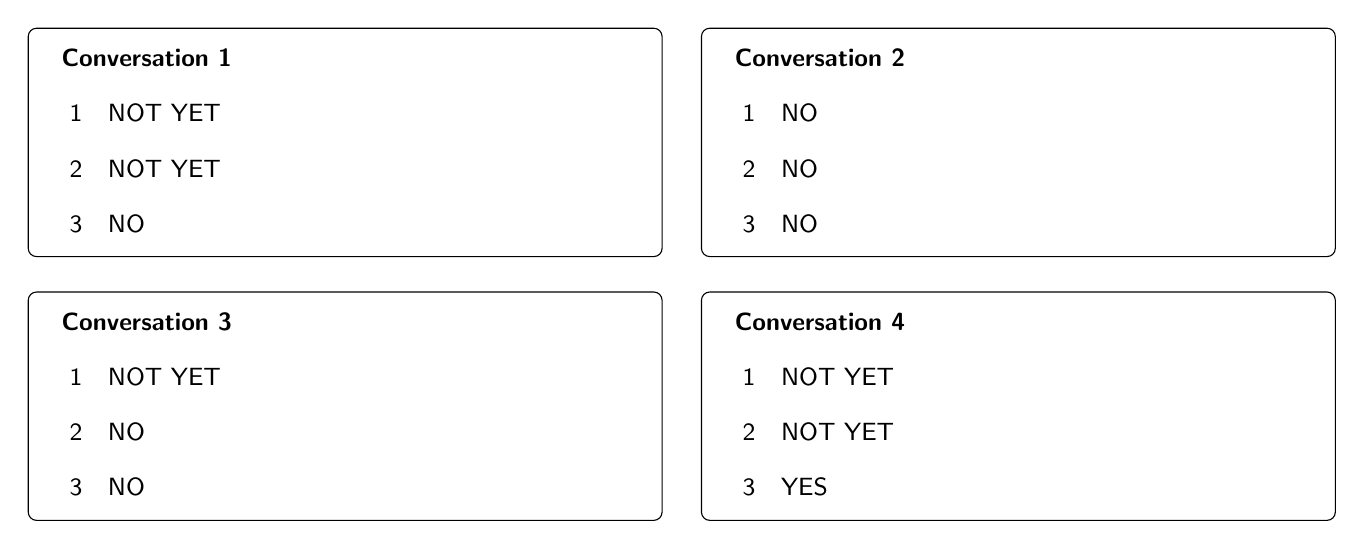
\begin{tikzpicture}[x=1cm,y=1cm]
 \transcript{0}{0}{1}{NOT YET}{NOT YET}{NO}
 \transcript{8.55}{0}{2}{NO}{NO}{NO}
 \transcript{0}{-3.35}{3}{NOT YET}{NO}{NO}
 \transcript{8.55}{-3.35}{4}{NOT YET}{NOT YET}{YES}
\end{tikzpicture}
\end{center}
\newpage
Each doll wears B (blue) or R (red), sees the other dolls' headbands and cannot see its own. Everyone hears: ``At least one headband is blue.''

A doll shows PROVE BLUE only when every possible arrangement matching what it sees gives it a blue headband. Otherwise it shows NOT YET.

A doll's matching cards are a temporary private view. Leave the shared set unchanged while choosing all three replies. Reveal replies together. Then remove arrangements that could not give those replies. Keep the headbands unchanged.

With two dolls, match a doll's view to the possibility cards:
\begin{center}
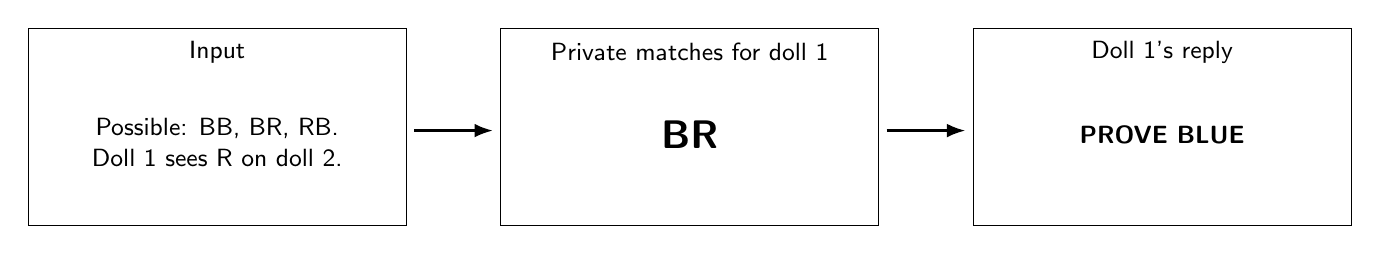
\begin{tikzpicture}[x=1cm,y=1cm,>=Latex]
 \draw (0,0) rectangle (4.8,2.5);\draw (6,0) rectangle (10.8,2.5);\draw (12,0) rectangle (16.8,2.5);
 \node[font=\small] at (2.4,2.2) {Input};\node[font=\small] at (8.4,2.2) {Private matches for doll 1};\node[font=\small] at (14.4,2.2) {Doll 1's reply};
 \node[align=center,font=\small] at (2.4,1.05) {Possible: BB, BR, RB.\\Doll 1 sees R on doll 2.};
 \node[font=\Large\bfseries] at (8.4,1.15) {BR};
 \node[font=\small\bfseries] at (14.4,1.15) {PROVE BLUE};
 \draw[->,thick] (4.9,1.2)--(5.9,1.2);\draw[->,thick] (10.9,1.2)--(11.9,1.2);
\end{tikzpicture}
\end{center}

\problem{2}{Coach three dolls with each of these deals. Find their replies in each round until every blue doll can show PROVE BLUE. Start each deal with the eight headband cards, then use the shared announcement.}
\begin{center}
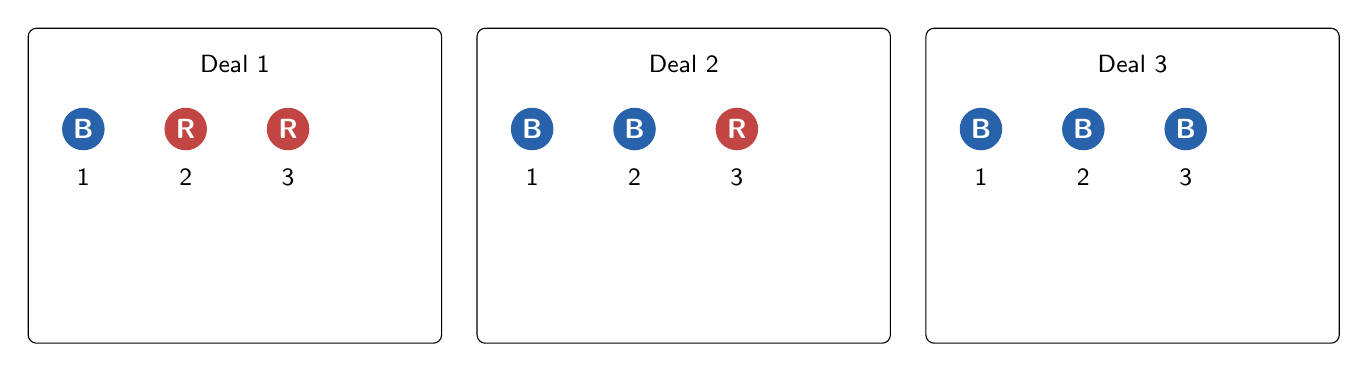
\begin{tikzpicture}[x=1cm,y=1cm]
 \foreach \x/\name in {0/1,5.7/2,11.4/3}{
  \draw[rounded corners=3pt] (\x,0) rectangle ++(5.25,-4.0);
  \node[font=\small] at (\x+2.625,-0.45) {Deal \name};
  \foreach \i in {1,2,3}{\node[font=\small] at ({\x+0.7+1.3*(\i-1)},-1.9) {\i};}}
 \hatdisk{0.7}{-1.28}{1}\hatdisk{2}{-1.28}{0}\hatdisk{3.3}{-1.28}{0}
 \hatdisk{6.4}{-1.28}{1}\hatdisk{7.7}{-1.28}{1}\hatdisk{9}{-1.28}{0}
 \hatdisk{12.1}{-1.28}{1}\hatdisk{13.4}{-1.28}{1}\hatdisk{14.7}{-1.28}{1}
\end{tikzpicture}
\end{center}
\newpage
\problem{3}{Start each trial with the announcement and all seven allowed headband cards. Put deals into groups that give the same three replies in round 1. Can later rounds separate every group?}
\vspace{2.7in}
\problem{4}{Use all eight headband cards and make no announcement. Can any doll ever show PROVE BLUE from these rounds? Settle it with the cards.}
\vfill
\newpage
\begin{center}
\begin{tikzpicture}[x=1in,y=1in]
\foreach \row/\one/\two/\three in {0/YES/YES/YES,1/YES/YES/NO,2/YES/NO/YES,3/YES/NO/NO,4/NO/YES/YES,5/NO/YES/NO,6/NO/NO/YES,7/NO/NO/NO}{
 \pgfmathtruncatemacro{\rr}{floor(\row/2)}\pgfmathtruncatemacro{\cc}{mod(\row,2)}
 \pgfmathsetmacro{\xx}{3.7*\cc}\pgfmathsetmacro{\yy}{-2.12*\rr}
 \draw[dashed] (\xx,\yy) rectangle ++(3.45,-1.85);
 \foreach \i/\word in {1/\one,2/\two,3/\three}{
  \node[font=\small] at ({\xx+0.58+1.13*(\i-1)},\yy-0.5) {\i};
  \node[font=\large\bfseries] at ({\xx+0.58+1.13*(\i-1)},\yy-1.15) {\word};}}
\end{tikzpicture}
\end{center}
\newpage
\begin{center}
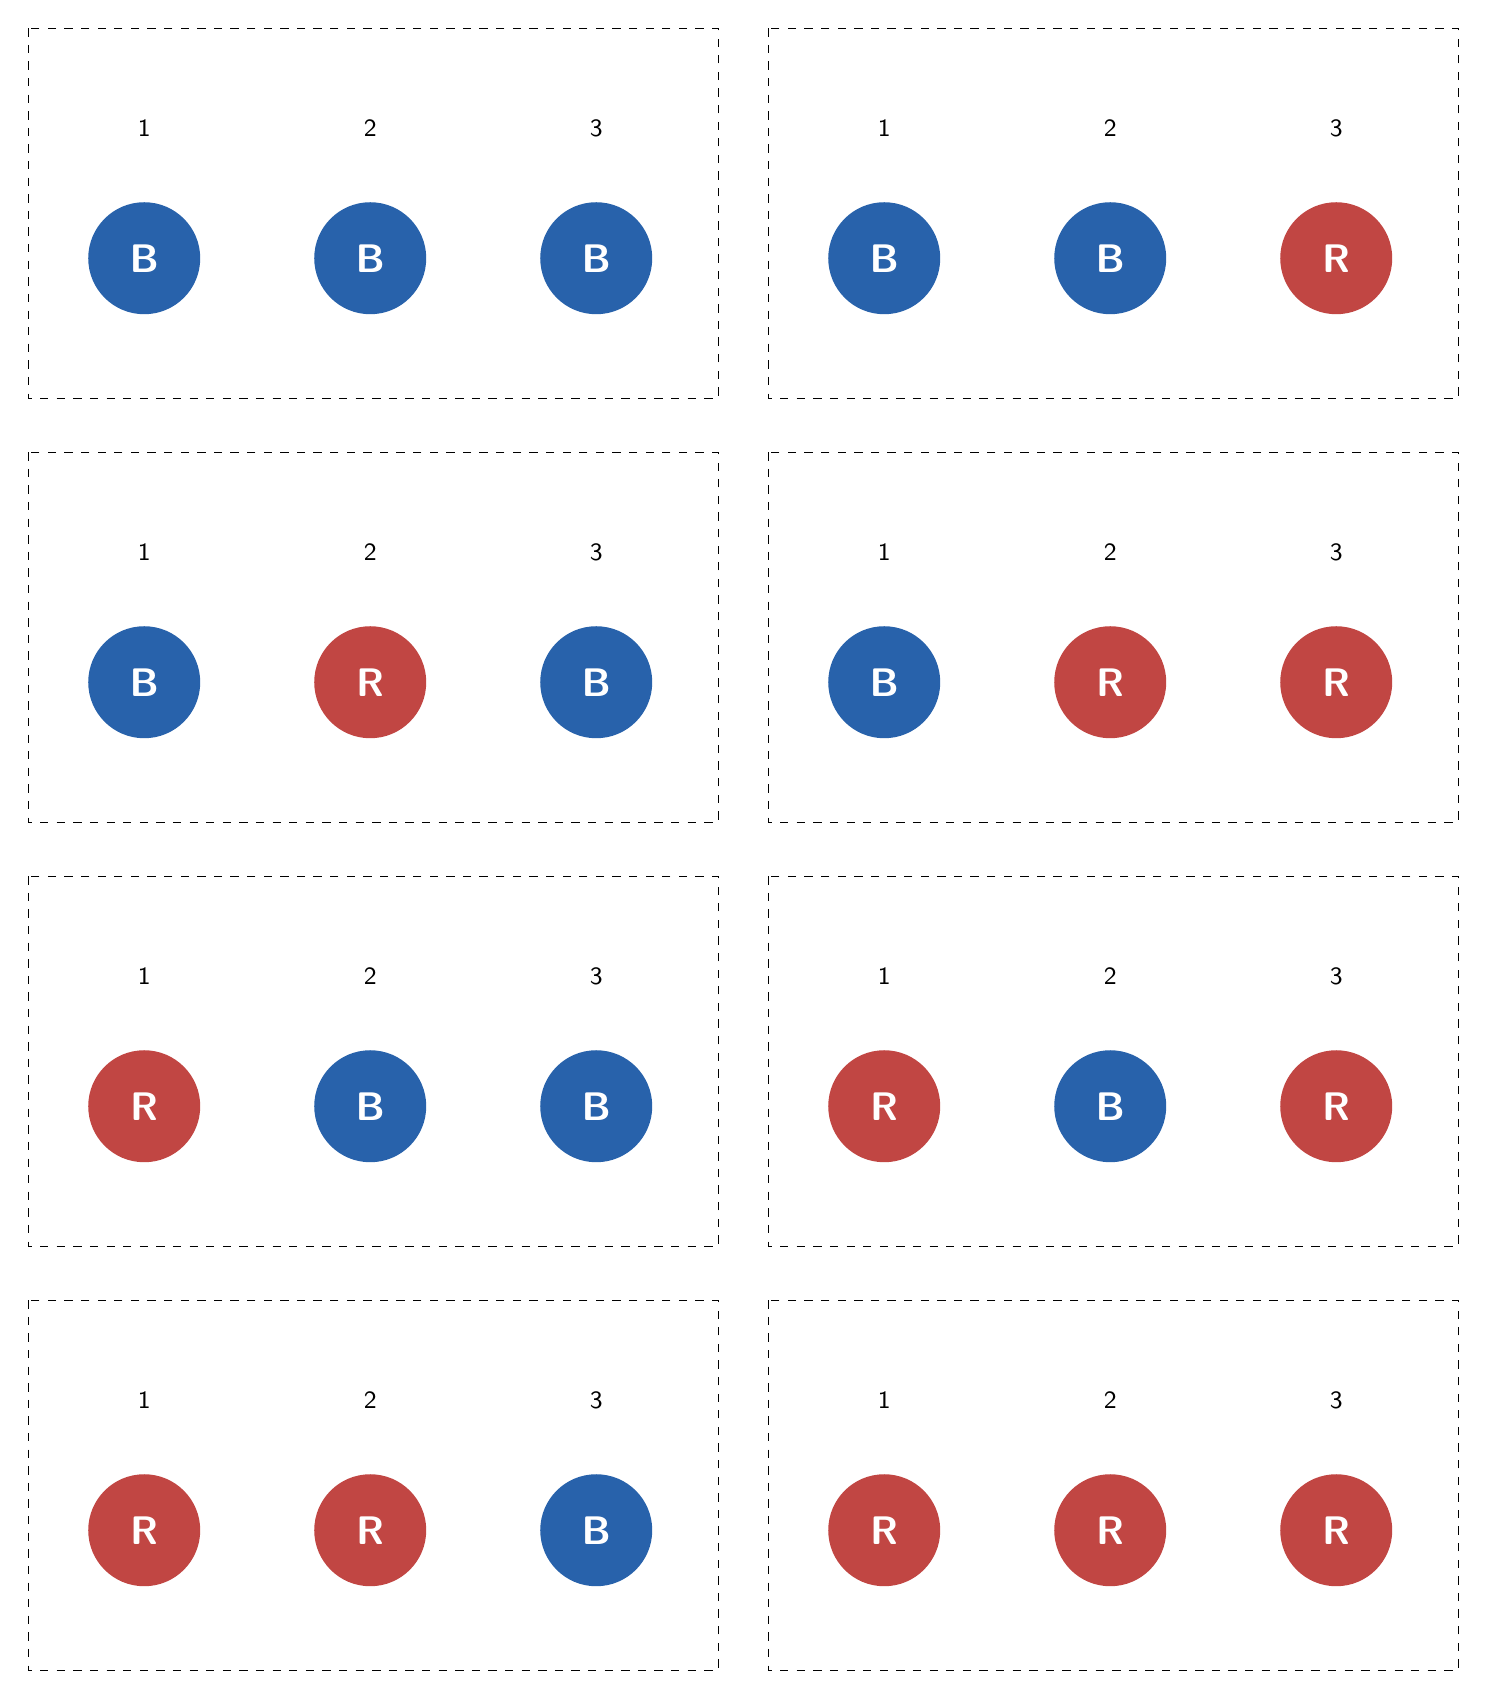
\begin{tikzpicture}[x=1in,y=1in]
\foreach \row/\one/\two/\three in {0/1/1/1,1/1/1/0,2/1/0/1,3/1/0/0,4/0/1/1,5/0/1/0,6/0/0/1,7/0/0/0}{
 \pgfmathtruncatemacro{\rr}{floor(\row/2)}\pgfmathtruncatemacro{\cc}{mod(\row,2)}
 \pgfmathsetmacro{\xx}{3.7*\cc}\pgfmathsetmacro{\yy}{-2.12*\rr}
 \draw[dashed] (\xx,\yy) rectangle ++(3.45,-1.85);
 \foreach \i/\val in {1/\one,2/\two,3/\three}{
  \node[font=\small] at ({\xx+0.58+1.13*(\i-1)},\yy-0.5) {\i};
  \ifnum\val=1\fill[hatblue] ({\xx+0.58+1.13*(\i-1)},\yy-1.15) circle (0.28);\node[text=white,font=\Large\bfseries] at ({\xx+0.58+1.13*(\i-1)},\yy-1.15) {B};
  \else\fill[hatred] ({\xx+0.58+1.13*(\i-1)},\yy-1.15) circle (0.28);\node[text=white,font=\Large\bfseries] at ({\xx+0.58+1.13*(\i-1)},\yy-1.15) {R};\fi}}
\end{tikzpicture}
\end{center}
\newpage
\begin{center}
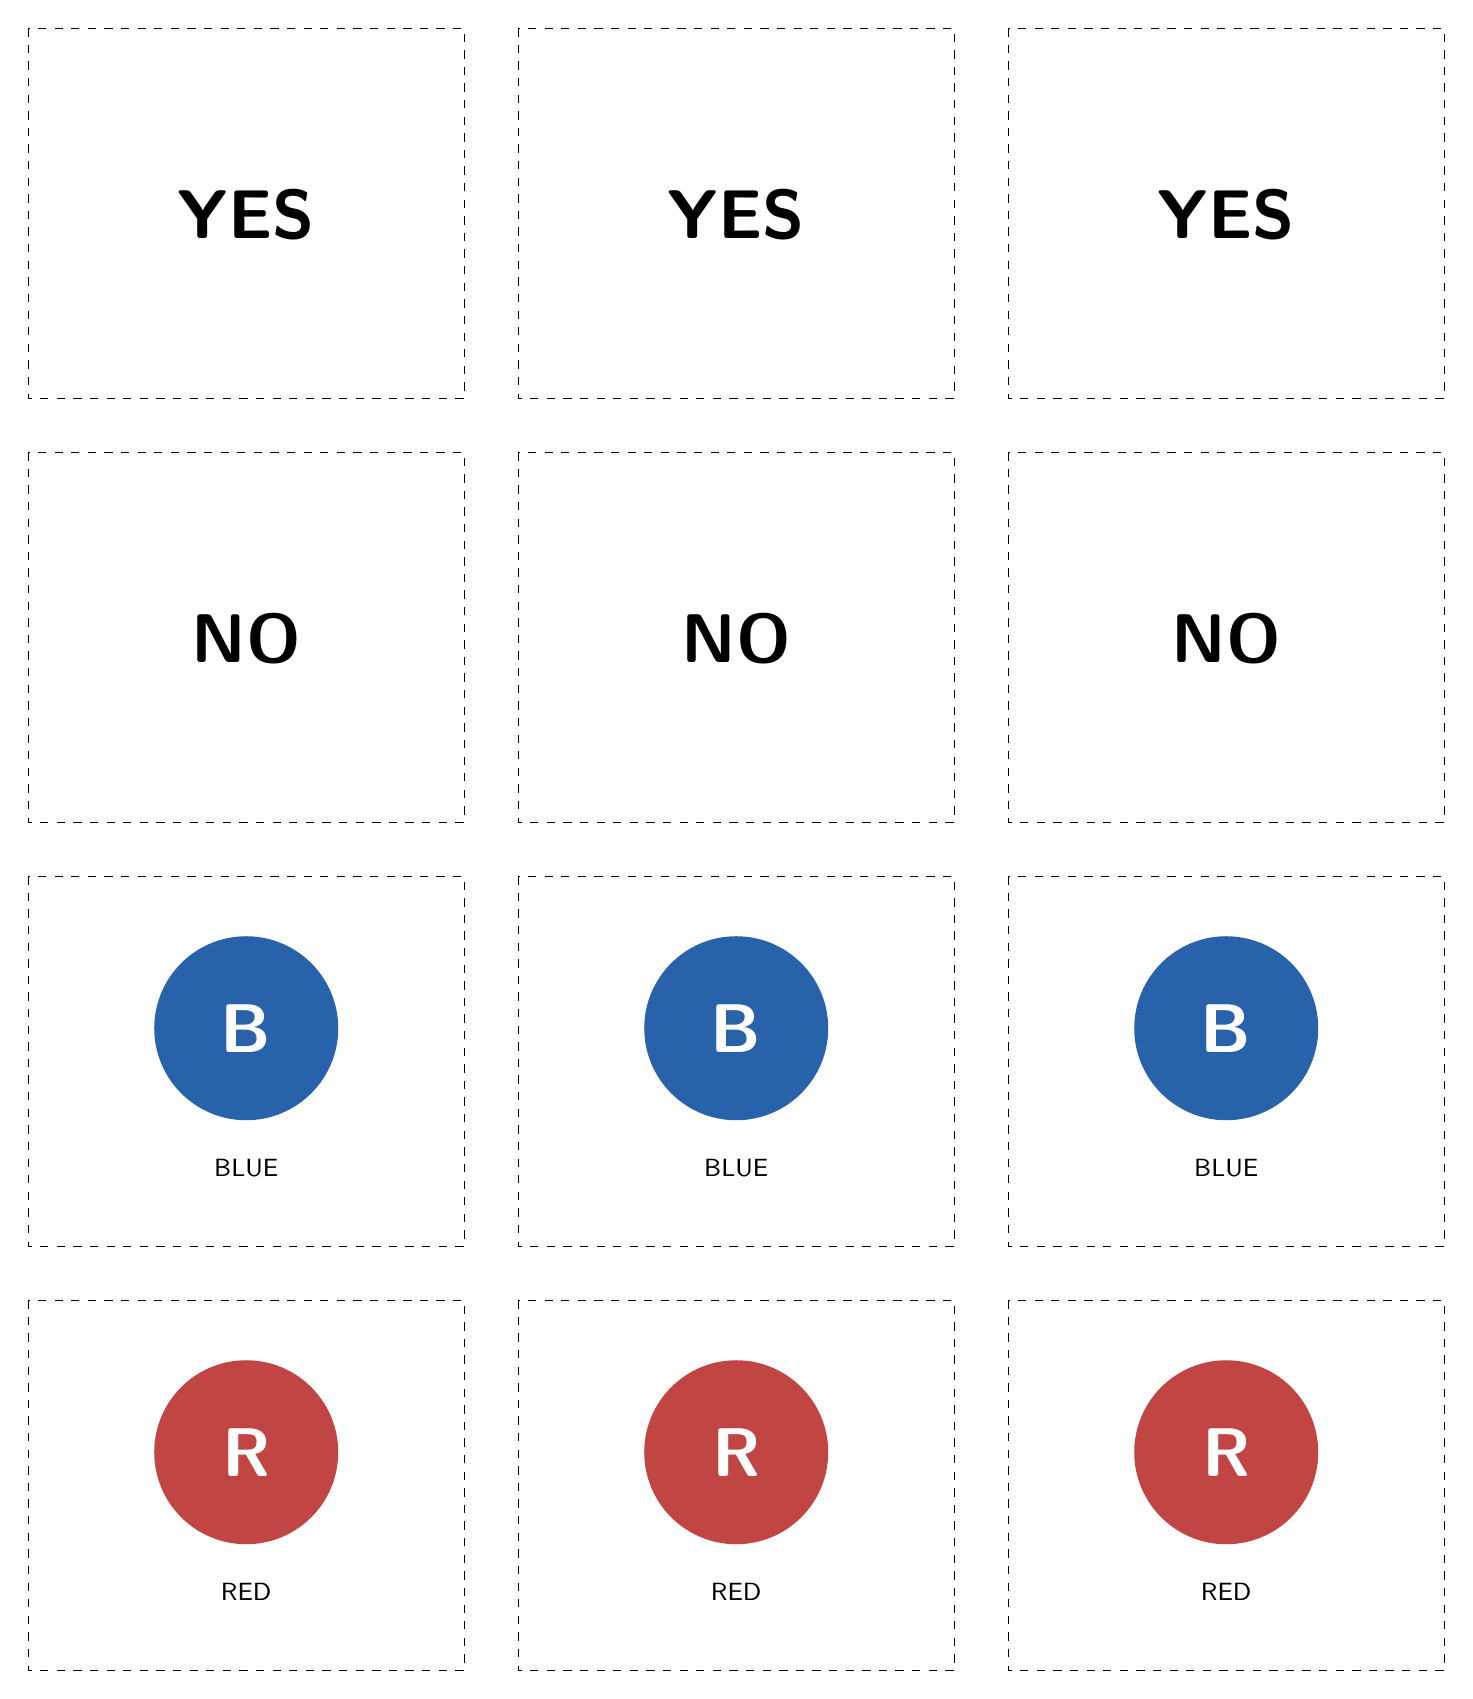
\begin{tikzpicture}[x=1in,y=1in]
\foreach \row/\word in {0/YES,1/YES,2/YES,3/NO,4/NO,5/NO,6/B,7/B,8/B,9/R,10/R,11/R}{
 \pgfmathtruncatemacro{\rr}{floor(\row/3)}\pgfmathtruncatemacro{\cc}{mod(\row,3)}
 \pgfmathsetmacro{\xx}{2.45*\cc}\pgfmathsetmacro{\yy}{-2.12*\rr}
 \draw[dashed] (\xx,\yy) rectangle ++(2.18,-1.85);
 \ifnum\row<6\node[font=\Huge\bfseries] at (\xx+1.09,\yy-0.93) {\word};
 \else\ifnum\row<9\fill[hatblue] (\xx+1.09,\yy-0.76) circle (0.46);\node[text=white,font=\Huge\bfseries] at (\xx+1.09,\yy-0.76) {B};\node[font=\small] at (\xx+1.09,\yy-1.46) {BLUE};
 \else\fill[hatred] (\xx+1.09,\yy-0.76) circle (0.46);\node[text=white,font=\Huge\bfseries] at (\xx+1.09,\yy-0.76) {R};\node[font=\small] at (\xx+1.09,\yy-1.46) {RED};\fi\fi}
\end{tikzpicture}
\end{center}
\newpage
\begin{center}
\begin{tikzpicture}[x=1in,y=1in]
\foreach \row/\word in {0/PROVE BLUE,1/PROVE BLUE,2/PROVE BLUE,3/NOT YET,4/NOT YET,5/NOT YET,6/YES,7/NO}{
 \pgfmathtruncatemacro{\rr}{floor(\row/3)}\pgfmathtruncatemacro{\cc}{mod(\row,3)}
 \pgfmathsetmacro{\xx}{2.45*\cc}\pgfmathsetmacro{\yy}{-2.65*\rr}
 \draw[dashed] (\xx,\yy) rectangle ++(2.18,-2.3);
 \node[align=center,text width=1.9in,font=\large\bfseries] at (\xx+1.09,\yy-1.15) {\word};}
\end{tikzpicture}
\end{center}
\newpage
\begin{center}
\begin{tikzpicture}[x=1in,y=1in]
 \draw[dashed] (0,0) rectangle (7.15,-0.85);
 \draw[dashed] (0,-1.25) rectangle (7.15,-2.1);
 \node[font=\Large\bfseries] at (3.575,-0.425) {Shared possibilities};
 \node[font=\Large\bfseries] at (3.575,-1.675) {Publicly ruled out};
 \foreach \i in {1,2,3}{
  \pgfmathsetmacro{\xx}{2.45*(\i-1)}
  \node[font=\large] at (\xx+1.09,-3.05) {Doll \i};
  \draw[rounded corners=3pt] (\xx,-3.4) rectangle ++(2.18,-2.3);}
\end{tikzpicture}
\end{center}
\end{document}
